\tikzset{
	circuit/.style={
		decorate, 
		double distance=4mm,
		decoration={
			snake, 
			pre length=4mm,
			post length=4mm,
			segment length=2.5mm,
			amplitude=.5mm,
		}
	},
	y/.pic={
		\draw[double distance=4mm] 
		(.5,0) -- ++(180:0.5) -- ++(+135:0.5) -- ++(180:0.2) coordinate (-C1)
		(.5,0) -- ++(180:0.5) -- ++(-135:0.5) -- ++(180:0.2) coordinate (-C2)
		;
		\coordinate (-PT) at(0.5,0);
	}
}

\begin{frame}{Déclenchement par débit}
	\begin{columns}
		\begin{column}{0.5\textwidth}
			\centering
			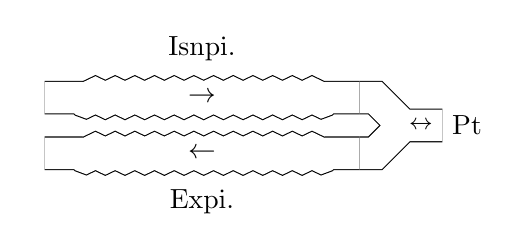
\begin{tikzpicture}[
					label distance=1.5mm
					]
				\pic (y){y};
				\draw [circuit] (y-C1) -- ++(-4cm,0) node[midway, label=above:Isnpi.] {$\rightarrow$};
				\draw [circuit] (y-C2) -- ++(-4cm,0) node[midway, label=below:Expi.] {$\leftarrow$};
				\node [right] at(y-PT) {Pt};
				\node [left, font=\footnotesize] at(y-PT) {$\leftrightarrow$};
			\end{tikzpicture}
		\end{column}
		\begin{column}{0.5\textwidth}
			\centering
			$\dot V_{I} - \dot V_{E} = \dot V_{pt}$
		\end{column}
	\end{columns}
\end{frame}
